\documentclass[12pt,a4paper]{article}

\usepackage{graphicx}
\usepackage{abstract}
\usepackage{hyperref}
\usepackage{listings}
\usepackage{amssymb}
%\usepackage{indentfirst}

\graphicspath{ {./images/} }
\renewcommand{\abstractname}{\large{Timestamps}}

\setlength{\parindent}{0.5in}

\title{CPSC 335 | Lecture \#3}
\author{Chris Nutter\thanks{Dedicated to @QuesoGrande a.k.a. Jared D.}}

% --> Here we go, satellite radio, y'all get hit with a...

\begin{document}

\maketitle

\begin{abstract}
    \noindent
    \begin{center}\textbf{09/14/2020 - 07:07:56 PM}\end{center}
        Read Ch. 3. It's about 30 pages. Could be important.\\
    \begin{center}\textbf{09/14/2020 - 07:44:53 PM}\end{center}
        Went to bathroom and lost information.\\
    \begin{center}\textbf{09/14/2020 - 07:44:53 PM}\end{center}
        Got back and Star said that he finished the problem.\\ 
    \begin{center}\textbf{09/14/2020 - 09:08:49 PM}\end{center}
        Read 3.4 \& 3.5. I mean theoretically read all sections cause \textbf{THE STUFF COULD BE ON THE TEST!!!}\\
\end{abstract}

\tableofcontents    

% -->

\section{After The Icosian Game}
    Directed Graph: Graph with directed edge\\\\
    $2^{20} = 1,000,000\\20! = 45,000,000\\$
    \begin{figure}[!hbtp]
        \centering
        \fbox{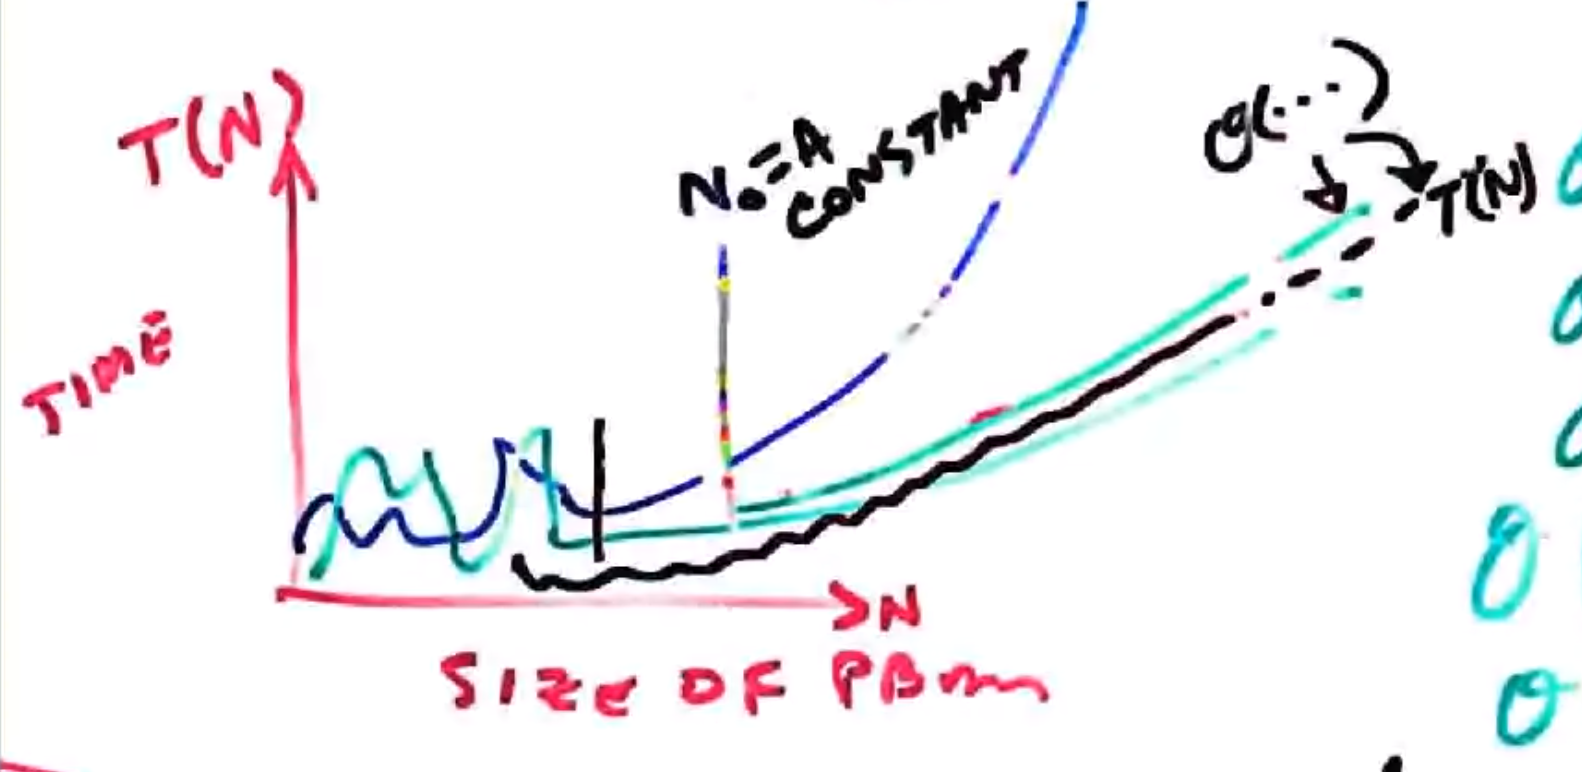
\includegraphics[width=13.8cm]{big_o.png}}
        \caption{Big(O) Notation}
    \end{figure}

    \begin{figure}[!hbtp]
        \centering
        \fbox{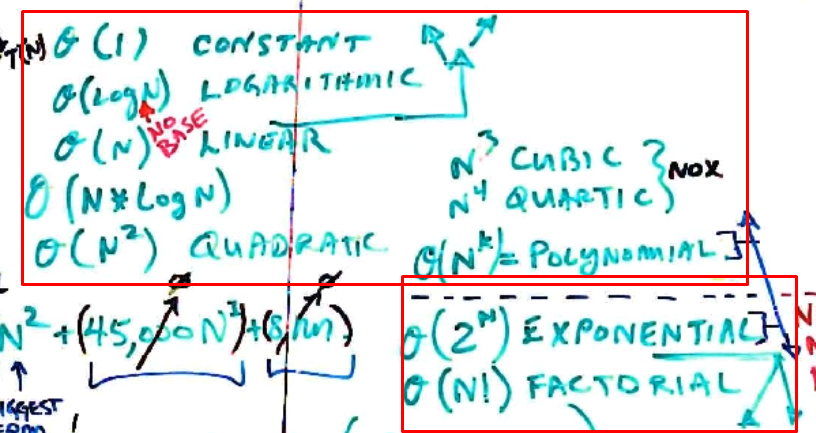
\includegraphics[width=13.8cm]{big_o-examples.png}}
        \caption{Big(O) Examples | \textbf{\emph{Important}}}
    \end{figure}

    \begin{figure}[!hbtp]
        \centering
        \fbox{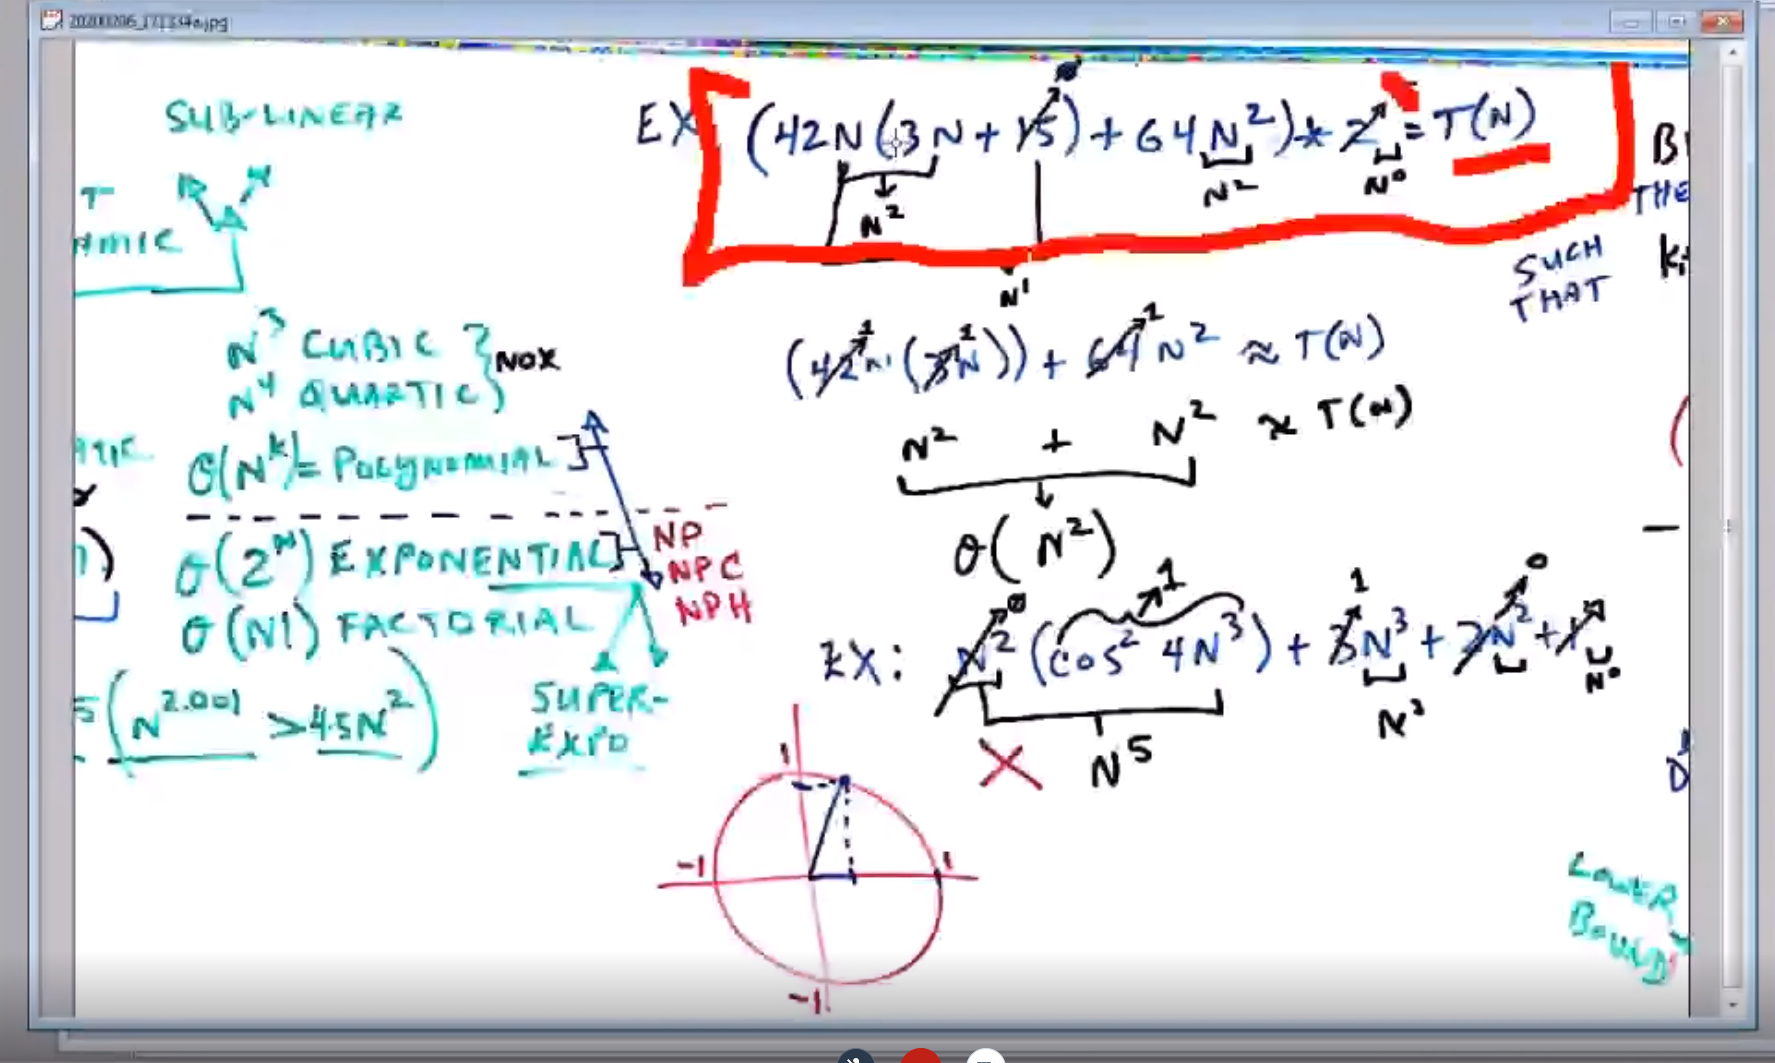
\includegraphics[width=13.8cm]{big_o-running-time.png}}
        \caption{Big(O) Running Times}
    \end{figure}

    \begin{figure}[!hbtp]
        \centering
        \fbox{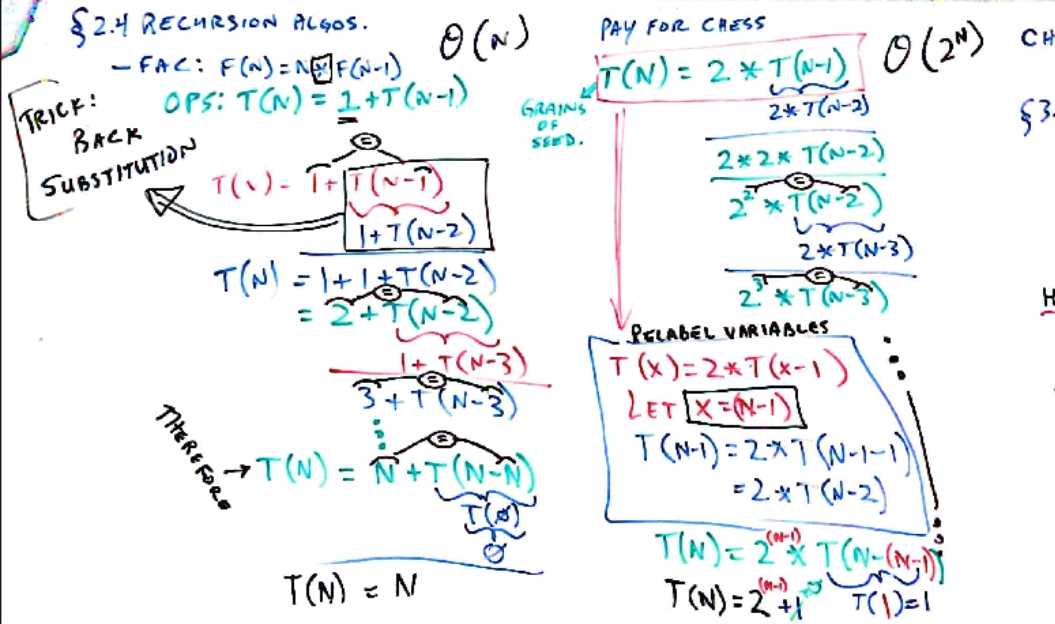
\includegraphics[width=13.8cm]{recursion-algo.png}}
        \caption{Recursion Algorithm}
    \end{figure}

\section{Chapter 3}
    \begin{figure}[!hbtp]
        \centering
        \fbox{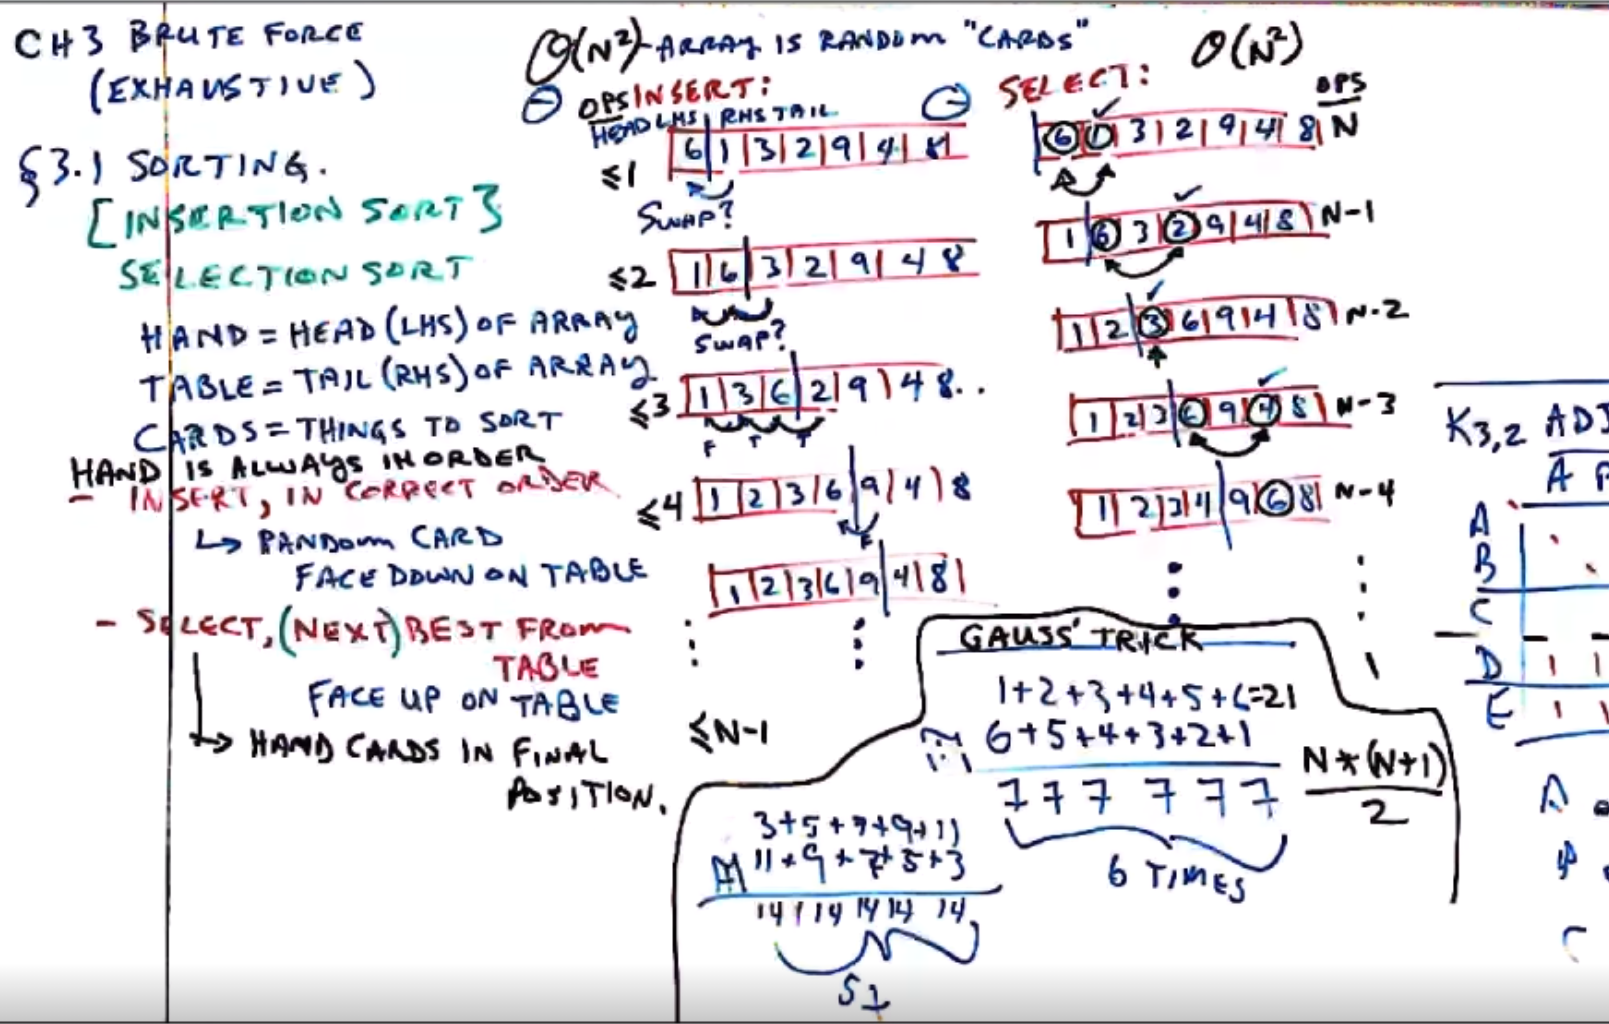
\includegraphics[width=13.8cm]{bruteforce.png}}
        \caption{Bruteforce Algorithm}
    \end{figure}

    \begin{figure}[!hbtp]
        \centering
        \fbox{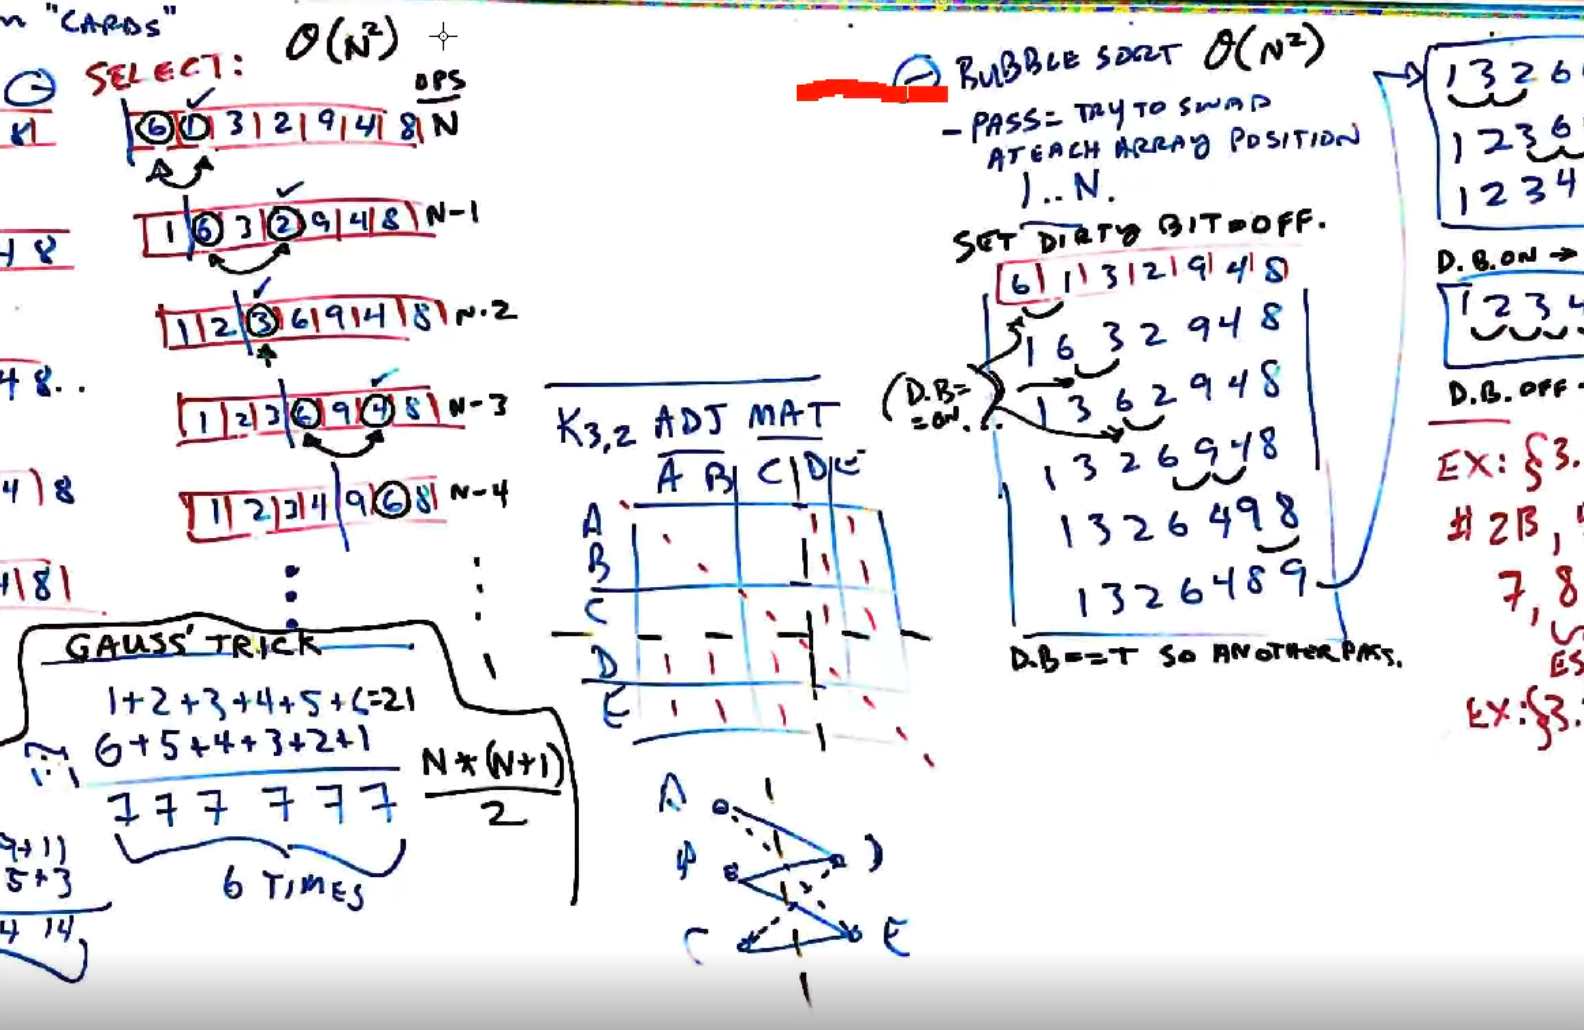
\includegraphics[width=13.8cm]{gauss-trick.png}}
        \caption{Gauss's Trick \& Bubble Sort}
    \end{figure}

    \begin{figure}[!hbtp]
        \centering
        \fbox{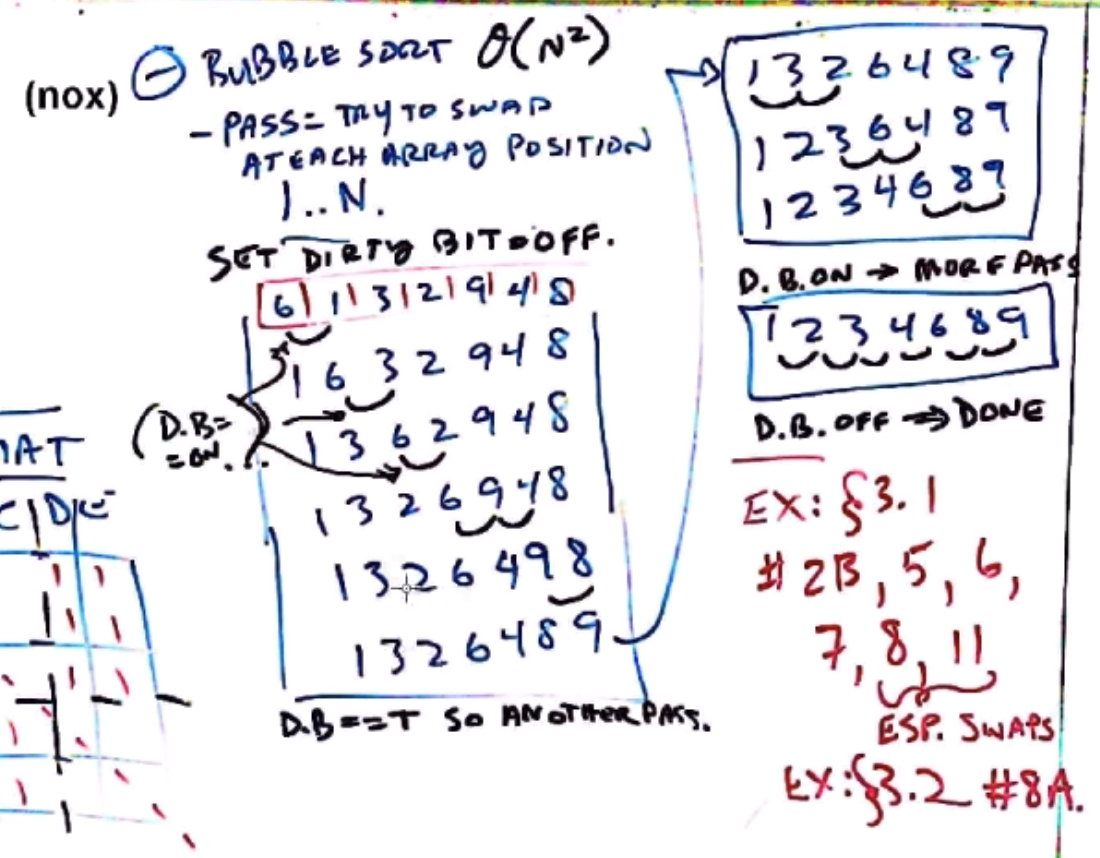
\includegraphics[width=13.8cm]{bubble-sort.png}}
        \caption{More Bubble Sort}
    \end{figure}

    \begin{figure}[!hbtp]
        \centering
        \fbox{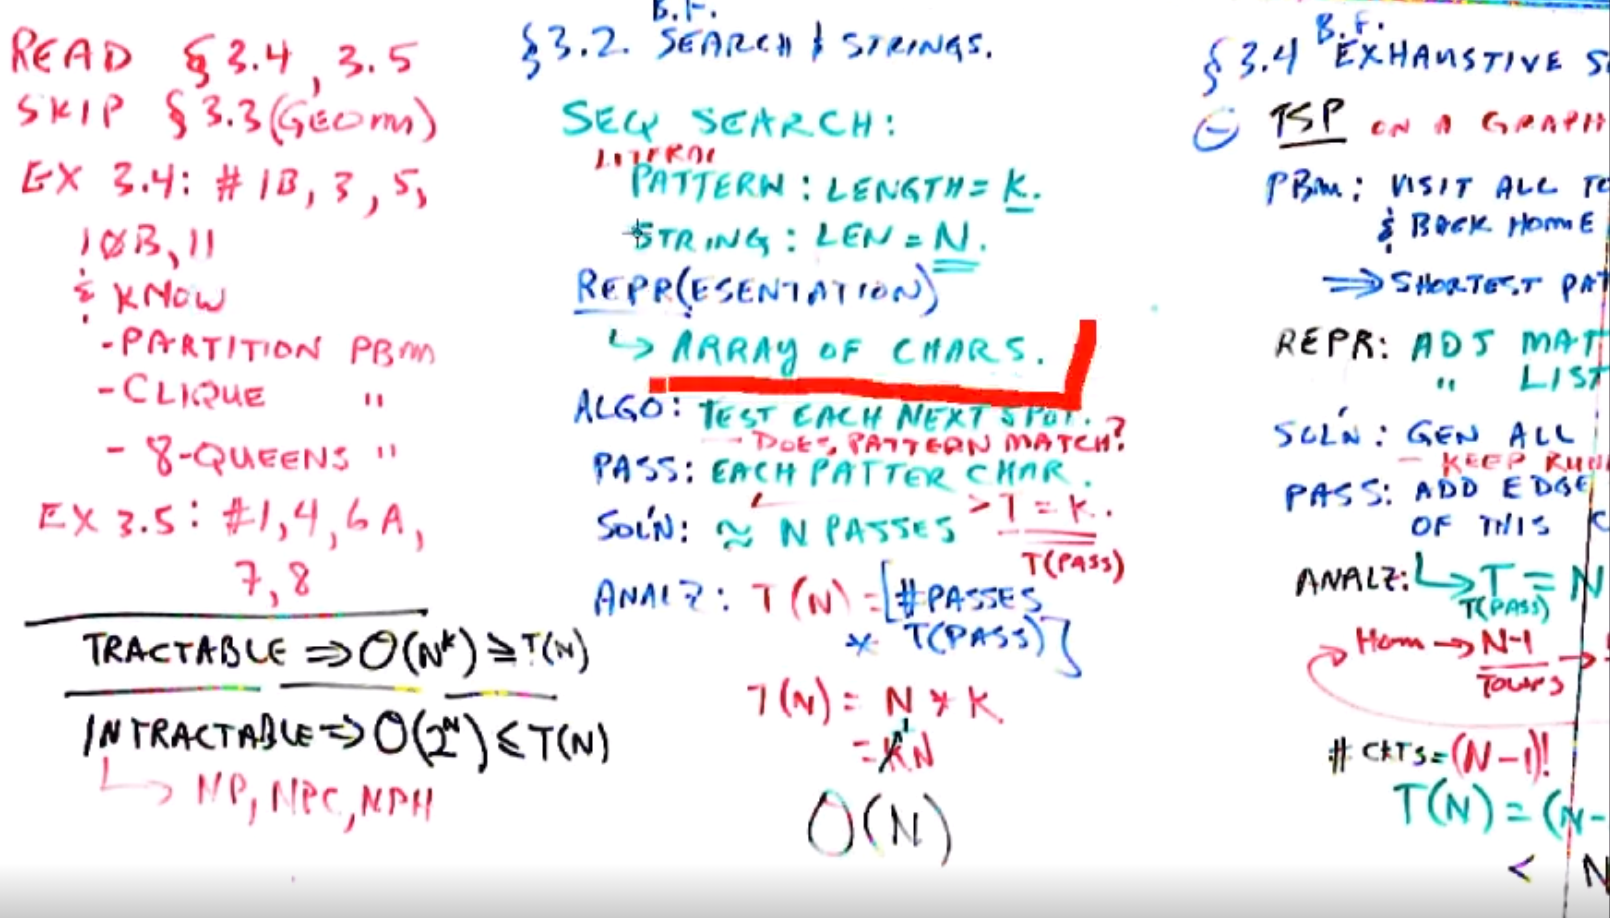
\includegraphics[width=13.8cm]{search+strings.png}}
        \caption{Search \& Strings}
    \end{figure}

    \begin{figure}[!hbtp]
        \centering
        \fbox{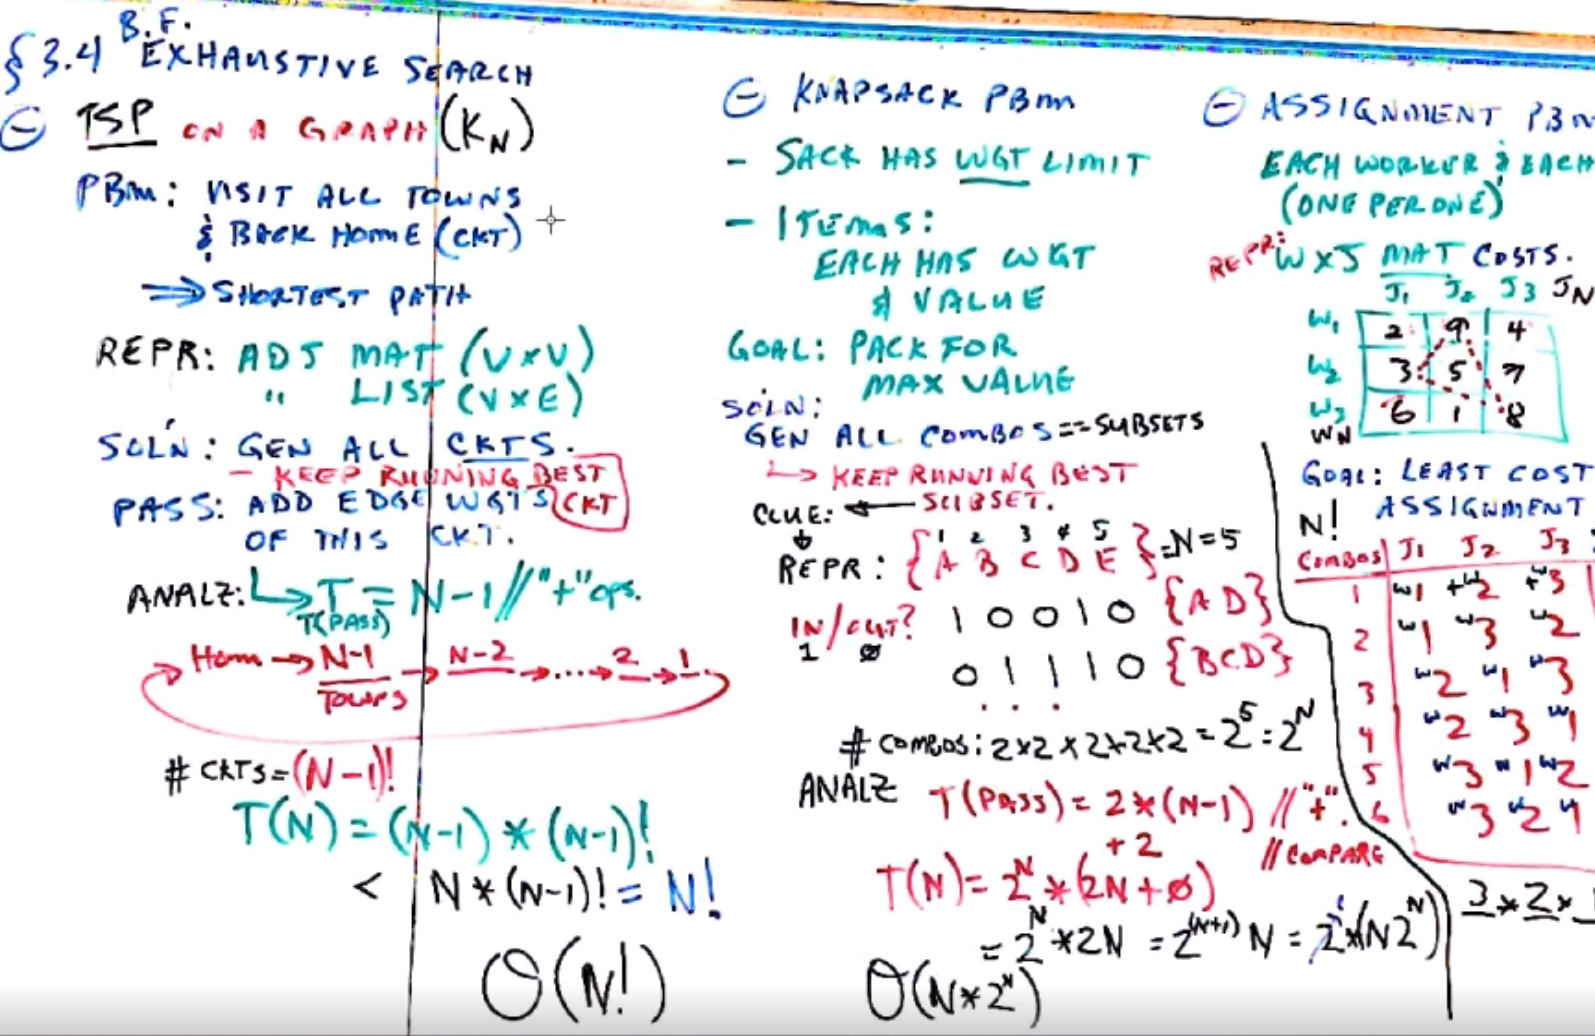
\includegraphics[width=13.8cm]{exhaustive-search.png}}
        \caption{Exhaustive Search, \textbf{TSP}: Traveling Salesman Problem}
    \end{figure}

\end{document} 
